% REMEMBER: You must not plagiarise anything in your report. Be extremely careful.

\documentclass{l4proj}

    
%
% put any additional packages here
%

\begin{document}

%==============================================================================
%% METADATA
\title{Implementing a Cryptocurrency}
\author{Sean Horgan}
\date{September 14, 2018}

\maketitle

%==============================================================================
%% ABSTRACT
\begin{abstract}
    \vskip 0.5em
    Over the past decade, cryptocurrency has become a rapidly growing area of interest as it aims to provide a 
    decentrilised alternative to regular fiat currencies. The goal of this project was to implement a peer-based 
    cryptocurrency. It is designed to include a distributed, tamper-proof ledger, a consensus mechanism 
    for distributing transactions to all participating nodes, a mining system, and wallets for sending 
    the currency between different addresses. It also includes a test harness so that a number of nodes 
    can be created and run on a single computer in order to test the system.
\end{abstract}

%==============================================================================

% EDUCATION REUSE CONSENT FORM
% If you consent to your project being shown to future students for educational purposes
% then insert your name and the date below to  sign the education use form that appears in the front of the document. 
% You must explicitly give consent if you wish to do so.
% If you sign, your project may be included in the Hall of Fame if it scores particularly highly.
%
% Please note that you are under no obligation to sign 
% this declaration, but doing so would help future students.
%
\def\consentname {Sean Horgan} % your full name
\def\consentdate {12 November 2019} % the date you agree
%
\educationalconsent


%==============================================================================
\tableofcontents

%==============================================================================
%% Notes on formatting
%==============================================================================
% The first page, abstract and table of contents are numbered using Roman numerals and are not
% included in the page count. 
%
% From now on pages are numbered
% using Arabic numerals. Therefore, immediately after the first call to \chapter we need the call
% \pagenumbering{arabic} and this should be called once only in the document. 
%
% Do not alter the bibliography style.
%
% The first Chapter should then be on page 1. You are allowed 40 pages for a 40 credit project and 30 pages for a 
% 20 credit report. This includes everything numbered in Arabic numerals (excluding front matter) up
% to but excluding the appendices and bibliography.
%
% You must not alter text size (it is currently 10pt) or alter margins or spacing.
%
%
%==================================================================================================================================
%
% IMPORTANT
% The chapter headings here are **suggestions**. You don't have to follow this model if
% it doesn't fit your project. Every project should have an introduction and conclusion,
% however. 
%
%==================================================================================================================================
\chapter{Introduction}

% reset page numbering. Don't remove this!
\pagenumbering{arabic} 

\section{Motivation}

The concept of cryptocurrency has only emerged in the past 15 years as an alternative to the regular,
centralised Fiat currencies backed by governments around the world. In 2008 Satoshi Nakamoto, the 
founder of Bitcoin, invented the worlds first cryptocurrency providing a peer-to-peer currency
not bound to a central bank. This new currency, secured by modern cryptographic methods, was a way in
which people around the world could trade without having to send the funds via a financial institution. (REFERENCE).

This new currency ensured security to its users by implementing a distributed ledger of transactions. Bitcoin
ensured that the ledger was immutable by ensuring proof of work was given before transactions would be
added to this ledger. This invention, known as the Blockchain, maintained security and prevented malicious
users from altering the system. The blockchain has become more than just a measure for ensuring security
in cryptocurrencies now though as it has become useful to thousands of companies around the world, being used
in hundereds of different contexts.

Bitcoin and other cryptocurrencies are much different to current fiat currencies as it is not tied to a physical
object like a note or coin. It is also immune to inflation as the value of currency in the system is dictated
by the proof of work system. This rewards nodes for mining blocks of transactions with a small amount of the 
currency. As the currency ages this reward is reduced until eventually there won't be any more given. This places
a limit on the total amount of the currency available.

\section{Goals}
The goal of this project is to create a secure and robust cryptocurrency from scratch. There are several key aspects
to the project that must be met in order to demonstrate a woking cryptocurrency.

The currency will be based around
a distrobuted ledger that is resistant to malicious retroactive changes. It will use a concept know as proof of work,
similar to the way that Bitcoin works where nodes have to solve difficult hashing calculations in order
to add transactions to the ledger. This concept is known as mining and is a way to make sure that transactions
are added at a steady rate while providing compensation to the node as an incentive to verify the transactions the node
is trying to add are valid and acceptable.

This cryptocurrency will include wallets with addresses allowing users to send any of their currency to another
wallet using its public key address. This will be shown in the test harness where a number of nodes and wallets 
will be created to simulate a populated network of users. A large number of emulated users will be required as on
smaller scales cryptocurrencies do not work perfectly and are succeptable to double-spending attacks where users
can spend more money than they own. The test harness should simulate a large active network by randomly creating
transactions from user to user to then be added on to the blockchain once the nodes have shown proof of work using 
the mining mechanism.

\section{Dissertation Outline}
The following dissertaiton is split into seven chapters as described below:
\begin{itemize}
    \item
        \textbf{Chapter 2} gives insight into the original Bitcoin paper and other features of cryptocurrencies
        created in the past.
    \item
        \textbf{Chapter 3} discusses the requirements gathering and analysis stage where the functionality
        of the project was decided.
    \item
        \textbf{Chapter 4} presents the way in which the cryptocurrency was designed, from the architecture of the blocks
        to the verification of transactions.
    \item
        \textbf{Chapter 5} highlights the way in which the projects was implemented, discussing the specific tools and 
        technologies used to create a secure cryptocurrency.
    \item
        \textbf{Chapter 6} discusses the evaluation of the projects. This shows how well the requirements were met, the
        performance of the system, and unit testing.
    \item
        \textbf{Chapter 7} concludes the project, summarising the project and reflecting on its execution. Here we also
        outline any future work that could be accomplished.
\end{itemize}


%==================================================================================================================================
\chapter{Background}
In this chapter we will discuss the background of the project. This will be presented by looking at the relevant research done by 
others that has similar goals to this project. We will also examine other cryptocurrencies created in the past that have aided 
in the completion of this project.


\section{Bitcoin white paper}
The first cryptocurrency to be created was Bitcoin. It was first presented in 2008 by Satoshi Nakamoto in the Bitcoin White Paper
titled "Bitcoin: A Peer-to-Peer Electronic Cash System". The concise 9 page article defines Nakamoto's method of preventing
double-spending attacks in a peer-to-peer currency without the need for a third party to act as a middle man. The creater
of Bitcoin wanted to avoid the use of a centralised mint as it can be seen as a single point of failure where every transaction
must be routed through. This places the whole trust of the network on the middle man and the company running this mint. 
Bitcoin avoids the need for a centralised middleman utilising modern cryptographic methods and technologies. This paper 
outlines the requirements for a functional cryptocurrency and as such was instrumental in guiding this project.

Below we describe the main funtionality presented in the Bitcoin white paper.


\subsection{Transactions}
The primary component of a cryptocurrency is a transaction between two users. In bitcoin this is described as being "a
chain of digital signatures". In this sense, a transaction is just a way of showing that ownership of the coin has
passed from the sender's address to the recipient's address. Bitcoin ensures the immutability of these transactions
by making the sender generate a hash of the previous transaction combined with the public key, equivalent to the address,
of the recipient. This means that the recipient can then verify the transaction using their own key and the transaction
is confirmed as valid.

One issue with this method is that the recipient can validate that the transaction is correct but it cannot ensure
that the sender is double-spending the coin. Meaning the recipient cannot prevent the sender from also sending the 
same coin to another user. As Bitcoin was inteded to be a peer-to-peer currency with no centralised mint validating
all transactions and making sure there are no double spends, it is vital that there be some cryptographic method of
preventing these exploits.


\subsection{Blockchain}
The way Bitcoin achieves this validation without the need for a middleman is through the invention of the Blockchain.
The blockchain is described as a timestamp server which works by taking the hash of a block of data and publically
announcing this hash. This proves that the data exists at that time. Then the next block of data can include the
previous block's hash in it's own hash proving that both of these blocks of data existed at that time. This creates 
a chain of blocks which prove the order and time of creation.

This chain of blocks is extremely secure as it also protects against retroactive attacks. If a malicious user tries
to go back and alter a transaction in the blockchain then this would alter the hash of that block rendering it invalid,
this would then alter the next block's hash as each block's hash is a calculation using the hash of the previous block.
This would cascade through the whole blockchain invalidating every block from the point of the malicious change. The 
network would then recognise this chain is invalid and switch to a valid chain rendering the action of the malicious
user pointless.

\subsection{Consensus}
In order for the whole system of users to work, all nodes must agree on what is the correct blockchain to be using and
which blocks of transactions are to be added to the blockchain every time. This implemented in Bitcoin using a proof of
work mechanism. This system, also known as mining, means that in order for a node to add a block to the blockchain it
must find a value that, after being hashed, results in a number starting with a certain amount of '0's. This is 
effectivly setting a computational barrier to appending a block to the blockchain. This means that a certain amount of
CPU power is neseccary to append to the blockchain. This adds security to the system as it prevents singular malicious
users from hording IP addresses in order to take control of the network as theoretically the majority of computational
power in the network will be from benevolent users.

Because of this implementation of CPU power determining which blocks are added to the blockchain. It is easy for the
nodes to decide which blockchain to add their blocks to. They simply choose the longest blockchain as this will be
the blockchain with the most CPU power invested in it. This is secure as if an attacker were trying to alter a 
previous block they would also have to redo all the proof of work completed for every block after that in the chain.
It is infeasable as the attacker would have to complete the proof of work for these blocks extremely quickly in order
to outpace the community and become the longest chain before other nodes would start to use that blockchain.


\subsection{Blocks}
The final point relevent to this project mentioned in the Bitcoin white paper is the way that Bitcoin aimed to store
the transactions within the blocks in the blockchain. A simple method of storing these transactions in the block may
just be an unordered list. This would work as each transaction is unrelated to the other transactions in the block in
every way except perhaps the time it took place. This storage solution can be improved though by using a data structure
known as a merkle tree (REFERENCE). This data structure is a way in which to make the process of checking block validity
more efficient. The way Merkle trees work is by having every leaf node be the hash of the transaction it represents 
and every branch node is the hash of its two child nodes. This builds up a chain of hashes similar to the blockchain.
This means that in order for a node to check that a block is valid it only needs to check the root hash of the block as
if there were any altered transactions within the block that would have an avalanche effect up through the hashes
ultimately changing the root hash of the whole block.

Another benifit that the paper mentions of storing the transaction within the block this way is that it can lessen
the storage space needed to store each block. As the blocks can be validated using only their main hash. Nodes do 
not need to store every single transaction in the blockchain in order to confirm transactions relevent to itself.
Instead it can just store the main block hashes and save a large amount of storage. As Bitcoin becomes more and
more popular this is a big saving as the number of transactions grows larger and larger.

\begin{figure}
    \centering
    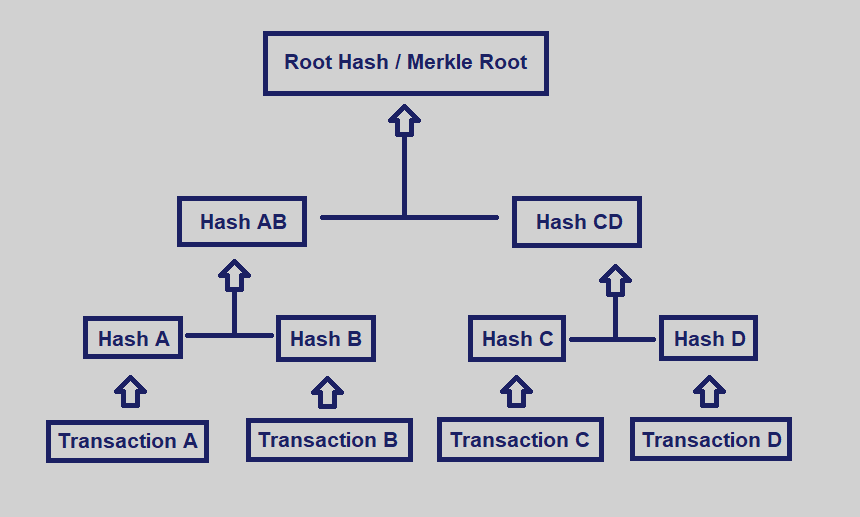
\includegraphics[width=0.7\linewidth]{images/merkle-tree.png}    

    \caption{
        The Merkle tree structure within a block of transactions. Transactions are hashed together as leaf nodes
        and repeated all the way up the tree to the main hash of the block, known as the Merkle root.
    }

    % use the notation fig:name to cross reference a figure
    \label{fig:relu} 
\end{figure}

\section{Bitcoin and Cryptocurrency Technologies}
A large source of the information used to plan this project and choose the relevant technologies to include was the
book \emph{Bitcoin and Cryptocurrency Technologies} by Narayanan et al. This provided a more in depth disscussion
about the intricacies of the structures needed for the project. The book also gives good information about cryptocurrencies
that were not Bitcoin which gave a bigger picture and provided options for doing things differently or ways to 
exclude areas of bitcoin that would not be relevant in the project.

\subsection{Flooding}
One of the key topics described in the book was ways for the nodes in the network to reach a consensus. This happens
multiple times during the running of a network. Once when nodes must identify and decide on which blockchain to use when
alternates appear. This is described by the Bitcoin white paper by picking the longest chain and distrobuting this to 
other nodes. It also happens when a new transaction occurs between two wallets, the transaction must be sent to all
nodes in order for the nodes to include it in their blocks so they can start mining the blocks to validate the transaction 
on the blockchain.

This method of flooding is explained in the book by showing that every node has a list of nearby nodes that is created
when it joins the network. Whenever a node recieves a transaction it first performs some checks and if it passes the 
checks, the transaction is propogated to all nodes on its nearby nodes list. First, the node checks if the transaction is
valid. It runs through the blockchain and checks that the funds the sender is trying to send actually belong to the sender.
Next, the node checks that the coins are not being double-spent, meaning the same funds have not already been sent to another
address perviously. Finally, the node checks if it has already seen the transaction, if it has it just disgards this new
transaction as the node will already have added it to a block. If the transaction passes all these test it is send to the
nearby nodes where it is put through the same tests until eventually it is spread to every node in the network or included
in a block on the blockchain.

\subsection{Mining}
One functionality described in the book is how mining changes over time. When a node mines a block that is included in the
blockchain they recieve a small reward which is an incentive to keep the blockchain updated. As explained perviously,
mining is the process of solving a hash calculation to result in a number starting with a certain number of '0's. The number
of 0s or target range, is changed over time. In Bitcoin, every 2016 blocks that are mined the difficulty of mining will be
altered. The way that this difficulty is altered depends on how quickly blocks were mined in the previous 2016 blocks. This
is done in order to maintain a consistant mining speed. The faster the nodes are mining blocks, the harder the difficulty
will subsequently become. As the network of users increases, the processing power increases and so the mining will happen
faster. This is also offset as over time the size of the incentive reward for successfully mining a block is lowered.
This reward system is the only way new coins are created and because of this there is a maximum to the total amount of coins
that will be in the system. This effectivly makes Bitcoin immune to inflation.

The way bitcoin automatically responds to changes in the amount of processing power and size of the network is impressive,
however will not be a useful addition to the project. As this project will run at a relativly small scale over a small
time span, it would not be utilised and would be unnecessary to include this feature.

\subsection{Bitcoin scripting}
Another major part of blockchain that the book describes is the small scripting languague that was invented specifically for
transactions which helps with the verification of transfers. This simple bitcoin scripting language is used
by nodes when mining blocks to verify that all transactions in the block are valid. Every transaction in Bitcoin is
sent with a script, most often instructing the node to compute the inputs of this transaction and the specified outputs of
previous transactions to make sure they match up correctly. Bitcoin also utilises this scripting language to inform the node
what the output should equal when the receiver tries to verify the transaction signature using their key. The book goes
into detail the intricacies of the language but this is out of scope for this project as including this scripting language
in the project would be unnecessary as there would only be one script needed and this can be implemented without the script.


%==================================================================================================================================
\chapter{Analysis/Requirements}
In this section we outline the exact nature of the project and how we gathered these requirements in order to 
complete the goals listed previously. We also discuss any functionality or features that have deliberatley been
left out of scope.

In this project the MoSCow method was used in order to prioritise the features so that the most important attributes
were included and some of the less important ones could be left to the end of the project to be added in if there was
time to spare.

\section{Functional Requirements}
Functional requirements listed here are features that must be included in the project in order for a woking,
useable cryptocurrency to be created. Without these requirements being met it would be impossible to carry out any
useful form of evaluation.

\subsection{Must have}
\begin{itemize}
    \item As described in the goals for the project, it would not constitute a cryptocurrency if it did not include a tamper-proof
        ledger for keeping track of all transactions between users. This must be resistant to malicious retroactive alterations
        and transactions that are invalid. This means that it must also have a feature so that nodes can run through the 
        whole chain and check all transactions are valid and each block links to the previous block.

    \item The cryptocurrency must also include some form of consensus mechanism where nodes can agree upon the blockchain
        and decide which transactions to include on the blockchain. They must be able to circulate each transaction once
        it occurs and flood it to other nodes on the network.
    
    \item Before blocks can be added to the blockchain it is important to inculde proof of work so that the integrity of the 
        networks blockchain can be maintained and guided by the processing power of the whole network and not a small minority
        of harmful nodes trying to take over.
\end{itemize}

\subsection{Should have}

A feature that can help with the smooth running of the network is an incentive for nodes to mine blocks. Without this there
is no reason for nodes to mine blocks and add to the blockchain. This is necessary as there needs to be a majority of 
honest nodes othewise it is easy for malicious nodes to take control of the blockchain and can then add any blocks with
which ever transactions they would like to the blockchain wether they are valid or not.

\subsection{Could have}
In Bitcoin, every 2016 blocks that are mined the difficulty of mining is changed in order to maintain the same average time
to mine a block. This difficulty is either made harder or easier based on how quickly the nodes mined the previous blocks.
This is not a high priority in this project as all the mining is taking place on the same computer and each node will have
the same computational power. In theory this means that the average time for mining blocks shouldn't change.

\section{Non-Functional Requirements}
Non-functional requiremnts are features that if included will improve the way the cryptocurrency operates by increasing
speed or lowering the storage space required. These features are not imperative to the operating of the cryptocurrency
but would bring the project closer to what might be used in current cryptocurrencies in the world at the moment.

\subsection{Must have}
It is important that the way in which the transactions within blocks is efficient. The must be stored using the Merkle
tree structure (REFERENCE). This way each transaction is a leaf node and every branch node is a hash of its two children.
This makes it extremely efficient for checking the validity of each block as you only have to check the hash of the root
hash.

\subsection{Should have}
The cryptocurrency should have the ability to split the balance of wallets such that if you send an amount but you only
have an increment of the currency larger than that amount then you should be sent back the value that you overpaid by.
For example if you start with 10 coins and you want to send 3 to another wallet you should be able to send your 10 coins
and recieve 7 back as overpay.

\subsection{Could have}
One feature that would save storage space would be the way in which transactions are stored in blocks. In the merkle tree
structure the transactions are hashed in order to speed up validation for nodes. This could be improved even more for 
nodes. It is possible that nodes only need to store the root hash of each block in order to do their validation as the
block hash is sufficient to check for incorrect transactions. This means each node can save a huge amount of storage space
by only storing each blocks root hash.

\section{Chosen Limitaions}
No bitcoin scripting
Nodes Expiring after a while. 



%==================================================================================================================================
\chapter{Design}
How is this problem to be approached, without reference to specific implementation details? 
\section{Guidance}
Design should cover the abstract design in such a way that someone else might be able to do what you did, but with a different language or library or tool.

%==================================================================================================================================
\chapter{Implementation}
What did you do to implement this idea, and what technical achievements did you make?
\section{Guidance}
You can't talk about everything. Cover the high level first, then cover important, relevant or impressive details.



\section{General points}

These points apply to the whole dissertation, not just this chapter.



\subsection{Figures}
\emph{Always} refer to figures included, like Figure \ref{fig:relu}, in the body of the text. Include full, explanatory captions and make sure the figures look good on the page.
You may include multiple figures in one float, as in Figure \ref{fig:synthetic}, using \texttt{subcaption}, which is enabled in the template.



% Figures are important. Use them well.
\begin{figure}
    \centering
    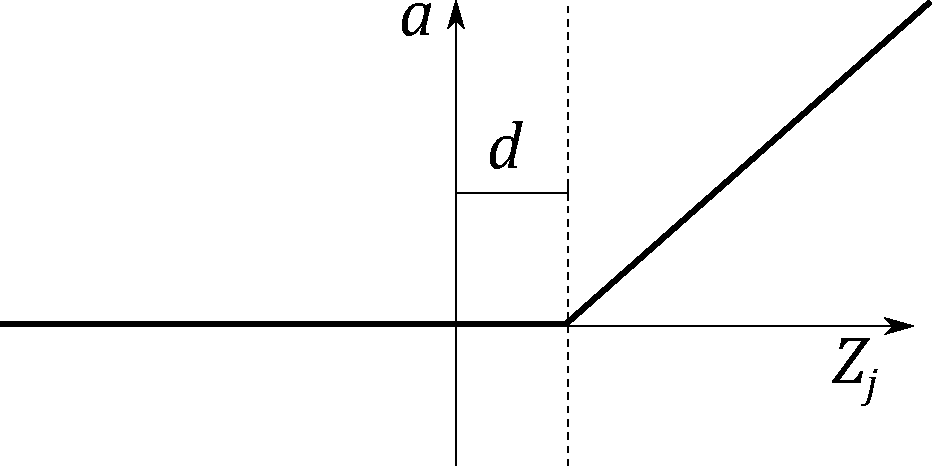
\includegraphics[width=0.5\linewidth]{images/relu.pdf}    

    \caption{In figure captions, explain what the reader is looking at: ``A schematic of the rectifying linear unit, where $a$ is the output amplitude,
    $d$ is a configurable dead-zone, and $Z_j$ is the input signal'', as well as why the reader is looking at this: 
    ``It is notable that there is no activation \emph{at all} below 0, which explains our initial results.'' 
    \textbf{Use vector image formats (.pdf) where possible}. Size figures appropriately, and do not make them over-large or too small to read.
    }

    % use the notation fig:name to cross reference a figure
    \label{fig:relu} 
\end{figure}


\begin{figure}
    \centering
    \begin{subfigure}[b]{0.45\textwidth}
        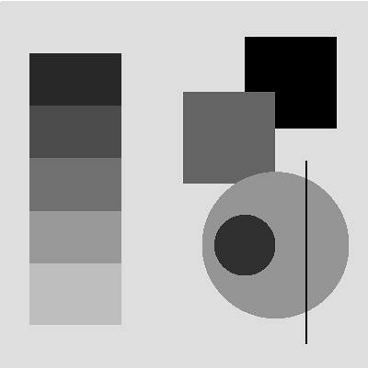
\includegraphics[width=\textwidth]{images/synthetic.png}
        \caption{Synthetic image, black on white.}
        \label{fig:syn1}
    \end{subfigure}
    ~ %add desired spacing between images, e. g. ~, \quad, \qquad, \hfill etc. 
      %(or a blank line to force the subfigure onto a new line)
    \begin{subfigure}[b]{0.45\textwidth}
        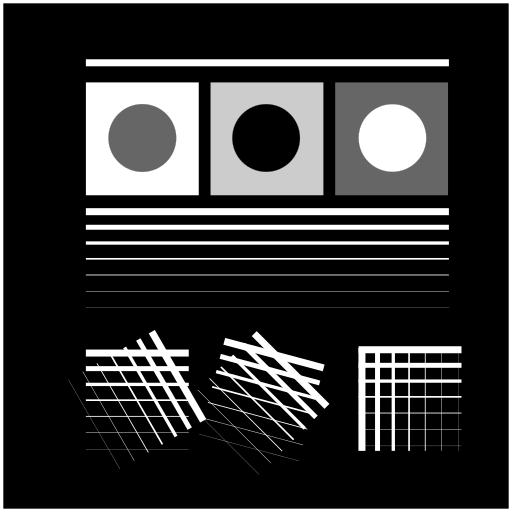
\includegraphics[width=\textwidth]{images/synthetic_2.png}
        \caption{Synthetic image, white on black.}
        \label{fig:syn2}
    \end{subfigure}
    ~ %add desired spacing between images, e. g. ~, \quad, \qquad, \hfill etc. 
    %(or a blank line to force the subfigure onto a new line)    
    \caption{Synthetic test images for edge detection algorithms. \subref{fig:syn1} shows various gray levels that require an adaptive algorithm. \subref{fig:syn2}
    shows more challenging edge detection tests that have crossing lines. Fusing these into full segments typically requires algorithms like the Hough transform.
    This is an example of using subfigures, with \texttt{subref}s in the caption.
    }\label{fig:synthetic}
\end{figure}

\clearpage

\subsection{Equations}

Equations should be typeset correctly and precisely. Make sure you get parenthesis sizing correct, and punctuate equations correctly 
(the comma is important and goes \textit{inside} the equation block). Explain any symbols used clearly if not defined earlier. 

For example, we might define:
\begin{equation}
    \hat{f}(\xi) = \frac{1}{2}\left[ \int_{-\infty}^{\infty} f(x) e^{2\pi i x \xi} \right],
\end{equation}    
where $\hat{f}(\xi)$ is the Fourier transform of the time domain signal $f(x)$.

\subsection{Algorithms}
Algorithms can be set using \texttt{algorithm2e}, as in Algorithm \ref{alg:metropolis}.

% NOTE: line ends are denoted by \; in algorithm2e
\begin{algorithm}
    \DontPrintSemicolon
    \KwData{$f_X(x)$, a probability density function returing the density at $x$.\; $\sigma$ a standard deviation specifying the spread of the proposal distribution.\;
    $x_0$, an initial starting condition.}
    \KwResult{$s=[x_1, x_2, \dots, x_n]$, $n$ samples approximately drawn from a distribution with PDF $f_X(x)$.}
    \Begin{
        $s \longleftarrow []$\;
        $p \longleftarrow f_X(x)$\;
        $i \longleftarrow 0$\;
        \While{$i < n$}
        {
            $x^\prime \longleftarrow \mathcal{N}(x, \sigma^2)$\;
            $p^\prime \longleftarrow f_X(x^\prime)$\;
            $a \longleftarrow \frac{p^\prime}{p}$\;
            $r \longleftarrow U(0,1)$\;
            \If{$r<a$}
            {
                $x \longleftarrow x^\prime$\;
                $p \longleftarrow f_X(x)$\;
                $i \longleftarrow i+1$\;
                append $x$ to $s$\;
            }
        }
    }
    
\caption{The Metropolis-Hastings MCMC algorithm for drawing samples from arbitrary probability distributions, 
specialised for normal proposal distributions $q(x^\prime|x) = \mathcal{N}(x, \sigma^2)$. The symmetry of the normal distribution means the acceptance rule takes the simplified form.}\label{alg:metropolis}
\end{algorithm}

\subsection{Tables}

If you need to include tables, like Table \ref{tab:operators}, use a tool like https://www.tablesgenerator.com/ to generate the table as it is
extremely tedious otherwise. 

\begin{table}[]
    \caption{The standard table of operators in Python, along with their functional equivalents from the \texttt{operator} package. Note that table
    captions go above the table, not below. Do not add additional rules/lines to tables. }\label{tab:operators}
    %\tt 
    \rowcolors{2}{}{gray!3}
    \begin{tabular}{@{}lll@{}}
    %\toprule
    \textbf{Operation}    & \textbf{Syntax}                & \textbf{Function}                            \\ %\midrule % optional rule for header
    Addition              & \texttt{a + b}                          & \texttt{add(a, b)}                                    \\
    Concatenation         & \texttt{seq1 + seq2}                    & \texttt{concat(seq1, seq2)}                           \\
    Containment Test      & \texttt{obj in seq}                     & \texttt{contains(seq, obj)}                           \\
    Division              & \texttt{a / b}                          & \texttt{div(a, b) }  \\
    Division              & \texttt{a / b}                          & \texttt{truediv(a, b) } \\
    Division              & \texttt{a // b}                         & \texttt{floordiv(a, b)}                               \\
    Bitwise And           & \texttt{a \& b}                         & \texttt{and\_(a, b)}                                  \\
    Bitwise Exclusive Or  & \texttt{a \textasciicircum b}           & \texttt{xor(a, b)}                                    \\
    Bitwise Inversion     & \texttt{$\sim$a}                        & \texttt{invert(a)}                                    \\
    Bitwise Or            & \texttt{a | b}                          & \texttt{or\_(a, b)}                                   \\
    Exponentiation        & \texttt{a ** b}                         & \texttt{pow(a, b)}                                    \\
    Identity              & \texttt{a is b}                         & \texttt{is\_(a, b)}                                   \\
    Identity              & \texttt{a is not b}                     & \texttt{is\_not(a, b)}                                \\
    Indexed Assignment    & \texttt{obj{[}k{]} = v}                 & \texttt{setitem(obj, k, v)}                           \\
    Indexed Deletion      & \texttt{del obj{[}k{]}}                 & \texttt{delitem(obj, k)}                              \\
    Indexing              & \texttt{obj{[}k{]}}                     & \texttt{getitem(obj, k)}                              \\
    Left Shift            & \texttt{a \textless{}\textless b}       & \texttt{lshift(a, b)}                                 \\
    Modulo                & \texttt{a \% b}                         & \texttt{mod(a, b)}                                    \\
    Multiplication        & \texttt{a * b}                          & \texttt{mul(a, b)}                                    \\
    Negation (Arithmetic) & \texttt{- a}                            & \texttt{neg(a)}                                       \\
    Negation (Logical)    & \texttt{not a}                          & \texttt{not\_(a)}                                     \\
    Positive              & \texttt{+ a}                            & \texttt{pos(a)}                                       \\
    Right Shift           & \texttt{a \textgreater{}\textgreater b} & \texttt{rshift(a, b)}                                 \\
    Sequence Repetition   & \texttt{seq * i}                        & \texttt{repeat(seq, i)}                               \\
    Slice Assignment      & \texttt{seq{[}i:j{]} = values}          & \texttt{setitem(seq, slice(i, j), values)}            \\
    Slice Deletion        & \texttt{del seq{[}i:j{]}}               & \texttt{delitem(seq, slice(i, j))}                    \\
    Slicing               & \texttt{seq{[}i:j{]}}                   & \texttt{getitem(seq, slice(i, j))}                    \\
    String Formatting     & \texttt{s \% obj}                       & \texttt{mod(s, obj)}                                  \\
    Subtraction           & \texttt{a - b}                          & \texttt{sub(a, b)}                                    \\
    Truth Test            & \texttt{obj}                            & \texttt{truth(obj)}                                   \\
    Ordering              & \texttt{a \textless b}                  & \texttt{lt(a, b)}                                     \\
    Ordering              & \texttt{a \textless{}= b}               & \texttt{le(a, b)}                                     \\
    % \bottomrule
    \end{tabular}
    \end{table}
\subsection{Code}

Avoid putting large blocks of code in the report (more than a page in one block, for example). Use syntax highlighting if possible, as in Listing \ref{lst:callahan}.

\begin{lstlisting}[language=python, float, caption={The algorithm for packing the $3\times 3$ outer-totalistic binary CA successor rule into a 
    $16\times 16\times 16\times 16$ 4 bit lookup table, running an equivalent, notionally 16-state $2\times 2$ CA.}, label=lst:callahan]
    def create_callahan_table(rule="b3s23"):
        """Generate the lookup table for the cells."""        
        s_table = np.zeros((16, 16, 16, 16), dtype=np.uint8)
        birth, survive = parse_rule(rule)

        # generate all 16 bit strings
        for iv in range(65536):
            bv = [(iv >> z) & 1 for z in range(16)]
            a, b, c, d, e, f, g, h, i, j, k, l, m, n, o, p = bv

            # compute next state of the inner 2x2
            nw = apply_rule(f, a, b, c, e, g, i, j, k)
            ne = apply_rule(g, b, c, d, f, h, j, k, l)
            sw = apply_rule(j, e, f, g, i, k, m, n, o)
            se = apply_rule(k, f, g, h, j, l, n, o, p)

            # compute the index of this 4x4
            nw_code = a | (b << 1) | (e << 2) | (f << 3)
            ne_code = c | (d << 1) | (g << 2) | (h << 3)
            sw_code = i | (j << 1) | (m << 2) | (n << 3)
            se_code = k | (l << 1) | (o << 2) | (p << 3)

            # compute the state for the 2x2
            next_code = nw | (ne << 1) | (sw << 2) | (se << 3)

            # get the 4x4 index, and write into the table
            s_table[nw_code, ne_code, sw_code, se_code] = next_code

        return s_table

\end{lstlisting}

%==================================================================================================================================
\chapter{Evaluation} 
How good is your solution? How well did you solve the general problem, and what evidence do you have to support that?

\section{Guidance}
\begin{itemize}
    \item
        Ask specific questions that address the general problem.
    \item
        Answer them with precise evidence (graphs, numbers, statistical
        analysis, qualitative analysis).
    \item
        Be fair and be scientific.
    \item
        The key thing is to show that you know how to evaluate your work, not
        that your work is the most amazing product ever.
\end{itemize}

\section{Evidence}
Make sure you present your evidence well. Use appropriate visualisations, reporting techniques and statistical analysis, as appropriate.

If you visualise, follow the basic rules, as illustrated in Figure \ref{fig:boxplot}:
\begin{itemize}
\item Label everything correctly (axis, title, units).
\item Caption thoroughly.
\item Reference in text.
\item \textbf{Include appropriate display of uncertainty (e.g. error bars, Box plot)}
\item Minimize clutter.
\end{itemize}

See the file \texttt{guide\_to\_visualising.pdf} for further information and guidance.

\begin{figure}
    \centering
    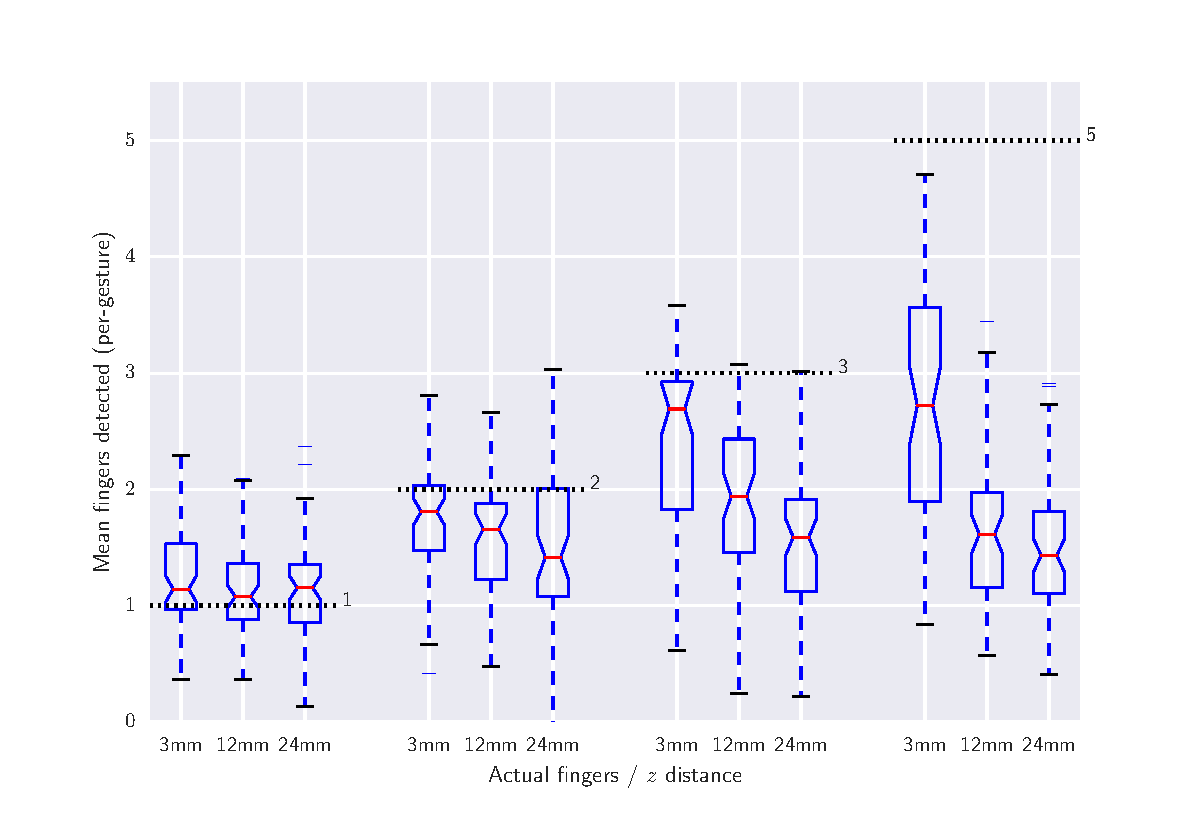
\includegraphics[width=1.0\linewidth]{images/boxplot_finger_distance.pdf}    

    \caption{Average number of fingers detected by the touch sensor at different heights above the surface, averaged over all gestures. Dashed lines indicate
    the true number of fingers present. The Box plots include bootstrapped uncertainty notches for the median. It is clear that the device is biased toward 
    undercounting fingers, particularly at higher $z$ distances.
    }

    % use the notation fig:name to cross reference a figure
    \label{fig:boxplot} 
\end{figure}


%==================================================================================================================================
\chapter{Conclusion}    
Summarise the whole project for a lazy reader who didn't read the rest (e.g. a prize-awarding committee).
\section{Guidance}
\begin{itemize}
    \item
        Summarise briefly and fairly.
    \item
        You should be addressing the general problem you introduced in the
        Introduction.        
    \item
        Include summary of concrete results (``the new compiler ran 2x
        faster'')
    \item
        Indicate what future work could be done, but remember: \textbf{you
        won't get credit for things you haven't done}.
\end{itemize}

\section{Future Work}

%==================================================================================================================================
%
% 
%==================================================================================================================================
%  APPENDICES  

\begin{appendices}

\chapter{Appendices}

Typical inclusions in the appendices are:

\begin{itemize}
\item
  Copies of ethics approvals (required if obtained)
\item
  Copies of questionnaires etc. used to gather data from subjects.
\item
  Extensive tables or figures that are too bulky to fit in the main body of
  the report, particularly ones that are repetitive and summarised in the body.

\item Outline of the source code (e.g. directory structure), or other architecture documentation like class diagrams.

\item User manuals, and any guides to starting/running the software.

\end{itemize}

\textbf{Don't include your source code in the appendices}. It will be
submitted separately.

\end{appendices}

%==================================================================================================================================
%   BIBLIOGRAPHY   

% The bibliography style is abbrvnat
% The bibliography always appears last, after the appendices.

\bibliographystyle{abbrvnat}

\bibliography{l4proj}
Merkle trees

Bitcoin white paper

Bitcoin and cryptocurrency technologies

https://hackernoon.com/merkle-trees-181cb4bc30b4
[IMAGE OF MERKLE TREE] 

\end{document}
